\chapter{Implementación}
\label{ch:chap04}

El siguiente capítulo encapsula los detalles de implementación y optimización de los algoritmos que se han desarrollado.

\section{OpenGL}
\label{sec:opengl-impl}

El algoritmo del hemi-cubo fue implementado utilizando la API OpenGL que provee de interfaces de alto nivel para la programación de tarjetas gráficas que facilitan el uso de algoritmos como el del Z-Buffer y facilita el manejo de memoria en la GPU.

\subsection{Cálculo de factores de forma de la componente difusa}
\label{sec:hemicubehgl}
Para implementar el cálculo de factores de forma se implementará la función \verb|computeFormFactors| como se aprecia en la figura \ref{img:procesado}. Recordando la arquitectura diseñada, la función debe computar completamente la matriz de factores de forma. Esta función seguirá un conjunto de etapas:

\begin{enumerate}
	\item En primera instancia, se configurarán los \textit{buffers} de memoria necesarios para representar el hemi-cubo que se dibujará.
	Para ello, se crea un \textit{Frame Buffer Object} en la GPU que estará compuesto de 5 texturas, cada una de ellas correspondiente a una de las caras a dibujar. Cabe destacar, que estas texturas se compondrán de dos imágenes, una de ellas contiene enteros sin signo que serán utilizados para representar un \verb|id| de cara parche de la escena y la restante contiene los valores de profundidad necesarios para el algoritmo del Z-Buffer.
	\item En la segunda se establecen las matrices de transformación de vista, es decir, las transformaciones lineales que alinean el volúmen de vista al hemicubo. Esto implica trasladar el origen de vista a el baricentro de la cara en cuestión, y alinearla a su normal como se ve en la figura.
	\item En la tercer etapa se procede a dibujar cada objeto en la escena desde el parche considerado en las cinco texturas que componen el hemi-cubo. Con el objetivo de tener el mejor rendimiento posible, se hace uso de los \textit{geometry shaders} para realizar una única llamada de dibujado por objeto. Este método solamente realiza un cambio de \textit{render target}, una de las operaciones más costosas según \ref{img:statechangescost}. Como puede apreciarse en \ref{alg:hemicube} solo se realiza una única llamada de \textit{binding} del hemi-cubo. Específicamente, la implementación sigue el siguiente patrón:
	\begin{enumerate}
		\item El \textit{vertex shader} es simplemente \textit{passthough} lo que signfica que conecta las entradas proveídas por la CPU con su salida.
		\item El \textit{geometry shader} genera cinco primitivas donde cada una estará en las coordenadas correspondientes a los frustums de las caras del hemicubo además de añadir un plano adicional de corte del dibujo necesario debido a la imposibilidad de que las caras laterales posean una resolución menor a la cara superior.
		\item El \textit{fragment shader} corregirá el identificador local \verb|gl_PrimitiveId| a un identificador global y escribirá el identificador de la cara detectada en la textura que le corresponda.
	\end{enumerate}
 \end{enumerate}

\begin{minipage}{\linewidth}
	\label{alg:hemicube}
	\begin{algorithmic}
		\Function{$processHemicube$}{$face, hemicube$}
			\State $row \gets [0,...,0]$
			\Loop{$ pixel \in hemicube:$}
				\State $factor \gets getHemicubeCorrection(pixel)$
				\State $seenFace \gets getFaceId(pixel)$
				\If{$isValid(seenFace)$}
					\State $row[seenFace] \gets + factor$
					\State $formFactorMatrix[face] \gets  row$
				\EndIf
			\EndLoop
		\EndFunction
		
		\Function{$computeFormFactors$}{}
			\State $bindHemicube()$
			\Loop{$face \in scene$}
				\State $alignCamera(face)$
				\State $clearBuffers()$
				\State $render(scene)$
				\State $hemicube \gets getHemicube()$
				\State $startThread(processHemicube, face, hemicube)$
			\EndLoop
		\EndFunction
		
	\end{algorithmic}
\end{minipage}

\vspace{5mm}
\begin{minipage}[h]{\linewidth}
	\centering
	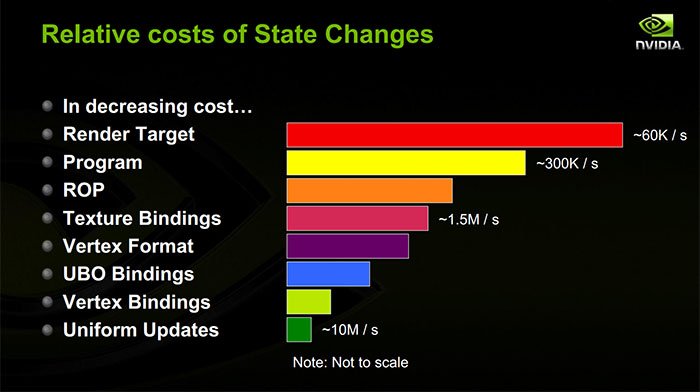
\includegraphics[width=\linewidth]{assets/statecosts}
	\captionof{figure}{Costo de cambios de estado en OpenGL. Fuente: Nvidia}
	\label{img:statechangescost}
\end{minipage}

\subsection{Cálculo de factores de forma de la componente especular}

El cálculo de factores de forma extendido en fue implementado en dos variantes para el método del hemi-cubo. Ambas variantes son métodos de "dos pasadas", es decir, se dibujará el hemicubo normalmente y luego de determinar qué caras visibles son reflectivas se computará el conjunto de caras visibles gracias a la reflexión.

Los métodos utilizados proveen \textbf{aproximaciones}, ya que al contrario de la técnica de trazado de rayos se desconoce el punto exacto en que los rayos emitidos desde el hemicubo colisionan con los parches del entorno.

La primer variante utiliza el método de dibujado de portales en la GPU, mientras que la segunda fue implementada utilizando \textit{trazado de rayos} en la CPU.

\subsubsection{Dibujado de portales}

El dibujado de portales es una técnica de dibujado en la rasterización en la que se dibujan únicamente los puntos cubiertos por cierta superficie (como una ventana, una puerta), normalmente se utiliza esta técnica para optimizar el dibujado de escenas donde la oclusión entre objetos es alta o la simulación de espejos planos.

Este método puede ser realizado de forma sencilla utilizando la GPU debido a los \verb|Stencil Buffers|, similares a los buffers de profundidad, pero almacenan información arbitraria que puede ser utilizada para decidir qué \textit{fragmentos} pasan la prueba del \verb|Stencil Test|.

En el caso de la implementación propuesta, el primer paso consiste en dibujar un \textit{stencil buffer} donde se encuentre el parche cuyo coeficiente de reflexión especular es mayor a cero desde la dirección simétrica como se aprecia en \ref{img:espejo}. Luego, manteniendo el mismo volúmen de vista, se dibujarán los identificadores de los parches de forma similar al dibujado del hemi-cubo en una textura bidimensional. Este proceso se realiza a una resolución muy baja con el objetivo de preservar el rendimiento y minimizar el costo de transferencia de memoria.

Finalmente, se obtienen los identificadores de las caras reflejadas. En caso de que existan caras con valores de reflexión mayor a cero se vuelven a procesar, en otro caso se utilizarán los identificadores obtenidos para distribuir el factor de forma correspondiente al píxel del hemi-cubo entre los parches visualizados.

\subsubsection{Trazado de rayos}

El algoritmo para el trazado es una <<traducción>> del algoritmo utilizando dibujado de portales. En este caso, se procederá de forma similar, salvo que en lugar de utilizar la rasterización para dibujar las caras desde el punto de vista simétrico, se trazarán rayos hacia la escena en la dirección de reflexión a partir de un conjunto de puntos distribuidos en el parche reflectivo.

\section{Embree}
\label{sec:embree-impl}

El algoritmo de la hemi-esfera fue implementado utilizando la biblioteca de traza de rayos Embree. Esta biblioteca soporta el trazado de rayos en la CPU en múltiples superficies, en particular, triángulos y cuadriláteros utilizando BHV (del inglés \textit{Bounding Volume Hirarchies}). Estas estructuras de datos se basan en árboles que sub-dividen la escena en cada nivel donde cada nodo corresponde a un volúmen que cubre un conjunto de primitivas en el cual el cálculo de las intersección rayo-BV tiene un costo computacional despreciable. Si la intersección rayo-BV no existe, es posible descartar todos los elementos que le preceden.

\subsection{Cálculo de factores de forma de la componente difusa}

De forma similar a \ref{sec:hemicubehgl} es necesario posicionar el origen de cada rayo a trazar en el baricentro de la superficie. Luego, recordando \eqref{ffhemiesfera}, es necesario generar un conjunto de direcciones utilizando la distribución del coseno o similar. Si bien originalmente se utilizó la generación de números pseudoaleatorios para generar rayos correctamente distribuidos, el uso de números aleatorios perjudicó el rendimiento del algoritmo. Es por esto que se decidió utilizar otro algoritmo de generación de direcciones pseudoaleatorias en una hemi-esfera, en este caso la \textit{regla general de particionado de una hemiesfera en celdas de área equitativa} propuesta por \citeauthor{Becker}.


Luego se procede a la traza de rayos, $\mathbf{F}_{ij}$ se calculará como $\frac{nIntersecciones_{ij}}{nMuestras}$, esto significa que por cada rayo que parta de la superficie $S_{i}$ impactando $S_{j}$ se adiciona $\frac{1}{nMuestras}$ al valor de la entrada correspondiente en $\mathbf{F}$.

\subsection{Cálculo de factores de forma de la componente especular}

En el caso del trazado de rayos, la extensión de los factores de forma es prácticamente trivial. Comprende la extensión de la función \verb|traceRay()| a devolver un conjunto de caras intersecadas. Básicamente, si el rayo inicial interseca una cara cuyo coeficiente de reflexión especular es estrictamente positivo se almacenará el total de $k(1 - \rho_{j})$ (donde $k = \frac{1}{nMuestras}$) como contribuyente del factor de forma $\mathbf{F}_{ij}$ y se calcularán las siguientes intersecciones con el \textit{residuo} de la reflexión que se distribuirá en los factores de forma que correspondan a la reflexión. Es decir, suponiendo que un rayo impacta $S_{k}$ desde el camino $(S_{i}, S_{j})$ donde $\rho_{j} \ge 0$ se agregará $k\rho_{j}*(1 - \rho_{k})$ y se procederá de forma recursiva hasta que $\rho_{z} = 0$ para una superficie intersecada $S_{z}$ o se alcance el máximo límite de recursión.

\section {Interfaz de usuario}

La interfaz de usuario fue implementada utilizando la bibioteca de dibujado de interfaces de usuario en modo inmediato \textit{ImGui}. Este método de dibujado implica que los comandos de dibujado de la interfaz se ejecutan inmediatamente y dependen del estado interno de la aplicación, este método era el utilizado en versiones anteriores de OpenGL o Direct3D.